\scanpage{151}
\mspage{75}

Let us prove a). Let \(\Gamma'\subset\mathcal E\) be
\inserted{a partial section over \(\Gamma_x\)}
deduced from \(x\in U^!\).
Let \(\Gamma''\supset\Gamma'_x\) be another \unsure{subgroup|subgroup}
\inserted{let \(\unsure{\Gamma_1}\supset\Gamma_x\) be its image \unsure{in|of} \(\Gamma\)}
such that \(\Gamma''\cap\pi=(1)\) i.e. \(\Gamma''\hookrightarrow\Gamma\)
\inserted{\illegible{1}}.
By the preceding theorem, it is defined by a unique
\unsure{\(y\in U^{\Gamma_1}\)|\(y\in U^{\Gamma''_*}\)},
and it is clear that this \(y\) does not change if we replace the action of
\(\unsure{\Gamma_1}\) on \(U\) by the action of a smaller group
\(\ne(1)\) (and the induced section) such as \(\Gamma_x\),
hence \(\unsure{\Gamma_1}\) \deleted{\illegible{1}} fixes \(x\) hence
(by definition of \(\Gamma_x\)) \(\Gamma_1=\Gamma_x\) hence
\(\Gamma''=\Gamma'\), \deleted{\unsure{q.e.d.}}

\deleted{\unsure{The injectivity}}\inserted{b)}
Let \(x,y\) give the same image
\([\Gamma']\ [\Gamma'']\), hence \(\Gamma_x=\Gamma_y\), say \(\Gamma_1\),
and applying the \unsure{theorem} to \(\Gamma_1\) operating on \(U\),
we find \(x=y\).
Let, on the other hand, \(\Gamma'_0\) be a maximal partial section \(\ne1\),
\(\Gamma_0\subset\Gamma\) its image,
by the theorem \inserted{applied to the action of \(\Gamma_0\) on \(U\),}
\(\exists x\in U\) \deleted{\unsure{fixed}} such that
\(x\in U^{\Gamma'_0}\) i.e. \(\Gamma'_0\subset\Gamma_x\),
and such that \([\Gamma'_0]\) is defined by \(x\),
but if \([\Gamma']\) is defined by \(x\) for the action of
\(\Gamma_x\) in its entirety, we will have \([\Gamma'_0]\subset[\Gamma']\),
hence by the maximal character of \([\Gamma'_0]\), we will have
\([\Gamma'_0]=[\Gamma']\), which \deleted{\illegible{1}} proves b).
On the other hand c) is clear.

\margin{150}

\scanpage{152}

Let us now return to the case where \(U=X\setminus S\), \(X\) a compact
\(T\)-oriented surface and \(S\) a finite
subset, anabelian case --- so we have a
\inserted{``fully} faithful'' description of \(U\) by a \(\pi\) with
loop structure, and we would like to convince ourselves
that \deleted{\illegible{2}} the \inserted{outer} operation of \(\Gamma\)
on \(\pi\), when \(\Gamma\) preserves orientation (to simplify)
also \unsure{suffices} to describe fully the object
\((U,\Gamma)\) in the appropriate isotopic category.
\margin{we should return to the general case for \unsure{what follows}\ldots}

We already recover a description of \(\unsure{U^!}\) in terms of
the action of \(\pi\), let \(J\) \inserted{\((\simeq U^!)\)},
the set of \(\pi\)-conjugacy classes
\deleted{moreover for every \(x\)}
of maximal partial sections \inserted{\(\ne1\)} of
\(\mathcal E\) over \(\Gamma\),
For every \(j\in J\), \(j\) is a \inserted{\(\pi\)-}torsor
as a
\inserted{\(\pi\)-}conjugacy class of sections
[that it is a \(\pi\)-torsor follows from
\(\pi^{\Gamma'}=(1)\), a priori
\deleted{\unsure{it is a \(\pi/\pi^{\Gamma'}\)-torsor}}
\inserted{\unsure{the stabilizer|the stabilizers} of \(\Gamma'\)}
is precisely \(\pi^{\Gamma'}\)]
In fact,

\margin{151}

\scanpage{153}
\mspage{76}

the set of \unsure{all} these \deleted{\unsure{classes}} maximal partial
sections is naturally an \(\mathcal E\)-set
(by conjugation) \deleted{\unsure{and}} on which \(\pi\) operates freely, and this
\(\mathcal E\)-set is canonically identified with
\(\widetilde U|U^!=\widetilde U^!\), for the structure of
\(\mathcal E\)-sets.

Let \(S'=S\cup U^!\), hence \(U'=X\setminus S'\),
we must try to reconstruct
(in terms of the extension \(\mathcal E\) of \(\Gamma\) by the group with
loops \(\pi\)) the \inserted{outer} group with loops corresponding
to \(\unsure{X'},S'\) i.e. to \(U'\), and the \deleted{extension}
\inserted{outer action} of \(\Gamma\) on it.
\deleted{\unsure{We hope to find a} \illegible{5}}
\deleted{\(\unsure{=}\) \illegible{5} \unsure{obvious}}

But first we should make sure of the intrinsic character of the
definition of \(J\) \unsure{\((\simeq U^!)\)|\((\simeq\widetilde U^!)\)}
\inserted{as a \(\Gamma\)-set,}
in terms of the \deleted{the action} \deleted{of the}
outer group \(\pi\), and of the outer action
\deleted{of \(\unsure{\Gamma}\)} of \(\Gamma\) on it.

\margin{152}

\scanpage{154}

This is rather obvious moreover
(in terms \inserted{precisely} of the
\inserted{\(\pi\)-}conjugacy classes of partial liftings of
\(\unsure{\Gamma\to\operatorname{Autext}(\pi)}\) to
\(\operatorname{Aut}(\pi)\)), we would however also like an
intrinsic description of \(\widetilde U|U^!\),
\unsure{in|or} a paradigm for the map of
\(\Gamma\)-spaces \(\unsure{U^!\longrightarrow U}\)
we must therefore describe a morphism of topoi with operation of \(\Gamma\) on it
\diagram{\begin{tikzcd}[ampersand replacement=\&]
B_J \arrow[r,"\unsure{\rho}"] \& B_{\unsure{\mathcal E}}
\end{tikzcd}}
which therefore corresponds to an \deleted{\unsure{morphism}} 
``inverse image'' functor \(\unsure{\rho^*|?^*}\)
(compatible with action of \(\Gamma\))
\deleted{\illegible{1}}
\diagram{\begin{tikzcd}[ampersand replacement=\&,row sep=2.5em,column sep=4em]
B_{\unsure{\mathcal E}} \arrow[r] \arrow[d,phantom,"\simeq"{description,rotate=90}] \& B_J \arrow[d,phantom,"\simeq"{description,rotate=90}] \\
\pi\text{-Sets} \& \mathrm{Ens.}\ \text{over }J
\end{tikzcd}}

This \deleted{\unsure{which}} is nothing other than the contracted product over
\(\pi\) with the set of maximal partial sections \(\ne1\) of
\(\mathcal E\) over \(\Gamma\)

\margin{153}

\scanpage{155}
\mspage{77}

Let us return to the extension \(\mathcal E\) of \(\Gamma\) by \(\pi\)
\deleted{\unsure{with faithful operation of \(\Gamma\)}}
arising from a geometric situation
(which extension, in the anabelian case, is already defined in terms
of an outer operation of \(\Gamma\) on \(\pi\))
we know that it satisfies additional
draconian conditions!
\inserted{\deleted{\unsure{to}} (To formulate them, we will assume the action of
\(\Gamma\) faithful):}
every subgroup \(\Gamma'\subset\mathcal E\) such that
\(\Gamma'\cap\pi=(e)\) (``partial section'') is
\inserted{cyclic (if \(\Gamma'=\Gamma'{}^0\)) or}
\deleted{\illegible{1}} dihedral,
\inserted{(if \(\Gamma'\ne\Gamma'{}^0\))}
and the set of \(\pi\)-conjugacy classes of such subgroups
is finite.
Every section subgroup \(\Gamma'\ne1\) is contained in a unique
\inserted{section} subgroup that is \uline{maximal}.
\margin{\unsure{good|so}
\figure{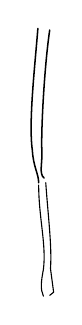
\begin{tikzpicture}[x=1mm,y=1mm,baseline=(current bounding box.center),line cap=round,line join=round]
\draw[line width=0.55pt] (0,34) .. controls (-0.4,29) and (-1.2,22) .. (-0.7,18.5) .. controls (-0.6,16.5) and (0.1,15.5) .. (0.1,14.4);
\draw[line width=0.40pt] (0.1,14.1) .. controls (0.1,10) and (1.1,6.5) .. (0.7,3.4) .. controls (0.4,1.8) and (0.3,0.9) .. (0.7,0);
\draw[line width=0.55pt] (1.5,33.8) .. controls (0.8,29) and (0.4,21) .. (0.5,18.5) .. controls (0.6,16.9) and (0.1,15.5) .. (0.8,15.0);
\draw[line width=0.40pt] (1.0,14.4) .. controls (1.3,10.1) and (1.8,6.3) .. (1.6,3.5) -- (2.0,0.5) -- (1.5,0.1);
\end{tikzpicture}}}

(We have established it at least in the case
\(\Gamma=\Gamma^0\), we should return to the general case,
I think it remains true as it stands, to be checked\ldots)
\margin{\figure{[A vertical stroke to the left of the two lines
``I think \ldots{} checked\ldots)''.]}}
Moreover, we saw an \uuline{additional structure} appear
on the group \(\mathcal E\)
[which in the anabelian case is identified with a subgroup of
\(\operatorname{Aut}(\pi)\)], namely a map
\[
\mu_{\mathcal E}:
\text{elements }\inserted{u}\text{ of finite order in }\mathcal E
\longrightarrow T\otimes\mathbb Q/\mathbb Z,
\]
\unsure{obtained} by noting that if \(u\in\mathcal E\) is of finite order
\(n\), \unsure{whence} \(\mathbb Z/n\mathbb Z\lhook\joinrel\xrightarrow[i]{}
\mathcal E\), \unsure{we have|i.e.} \(\operatorname{Im}i\cap\pi=(1)\)
(\(\pi\) has no torsion elements), hence
\(\mathbb Z/n\mathbb Z\hookrightarrow\Gamma\), \unsure{whence|of a} subgroup
\(\Gamma_1\subset\Gamma\) (i.e. the image of
\margin{\uline{N.B.} For a \(u\) of finite order in \(\mathcal E\),
we must \unsure{know|have}, if \(u\notin\mathcal E^0\),
that \(u\) \unsure{is} of order \(2\) exactly,
\illegible{5} to \unsure{define} \(\mu(u)\)!}

\margin{154}

\scanpage{156}

\(\unsure{u}\) in \(\Gamma\) has the same order \(n\)),
and the lifting \(\Gamma_1\hookrightarrow\mathcal E\) defines an
\(x\in U^{\Gamma_1}\), \deleted{such that} and \(u_1\) operating on \(U\)
while leaving \(x\) fixed therefore corresponds in a neighborhood of \(x\) to a
``multiplier'', which (for a chosen local orientation) is a
primitive \unsure{\(n\)th} root of \(1\) i.e. an element of
\(\mathbb Z/n\mathbb Z\), and which for varying orientation
is interpreted intrinsically as an element of
\(T\otimes\mathbb Z/n\mathbb Z
\subset T\otimes\mathbb Q/\mathbb Z\).

The map \(\mu\) satisfies the obvious conditions
\[
\begin{gathered}
\left\{
\begin{aligned}
\mu(\alpha u\alpha^{-1})&=\mu(u) &&\text{if }\alpha\in\pi\\
\mu(u^n)&=n\mu(u) &&\text{if }n\in\mathbb Z
\end{aligned}
\right.\\
\text{order }\mu(u)=\text{order of }u
\end{gathered}
\]
I do not know whether this map \(\mu\) \deleted{is}
\inserted{can be} defined intrinsically in terms of the extension
\(\mathcal E\), or whether on the contrary there can exist two extensions
\deleted{\unsure{isomorphic}} \(\mathcal E,\mathcal E'\) of \(\Gamma\) by \(\pi\),
defined by geometric situations, of \(\Gamma\) operating on
\(U\) resp. \(U'\), and an isomorphism of extensions
\(\mathcal E\longrightarrow\mathcal E'\) which is not compatible with
the functions \(\mu,\mu'\).
The simplest nontrivial case to look at is the

\margin{155}

\scanpage{157}
\mspage{78}

abelian case (where \(\pi\simeq\mathbb Z\)
\inserted{\deleted{\illegible{1}} \((\operatorname{card}I=2)\)}
or \(\pi\simeq\mathbb Z^2\) (\deleted{\unsure{cardinality}} \(I=\varnothing\))),
In the \inserted{first} case
\deleted{of an extension} \(\pi\simeq\mathbb Z\), \unsure{we|\deleted{the}}
\inserted{must have (to have a faithful action of
\(\Gamma=\Gamma^0\))}
\deleted{extensions \illegible{1}}
\(\Gamma^0\) cyclic, \(\mathcal E\simeq\mathbb Z\),
there is no element of finite order in \(\mathcal E\) except
\(\unsure{1|e}\), so the question does not arise.
The case \(\pi\simeq\mathbb Z^2\) is more interesting,
\deleted{\unsure{and can be reformulated}}

If \(\pi\) is a free \(\mathbb Z\)-module of
\deleted{\unsure{finite type}}\inserted{\unsure{rank \(n\)}}, we have an exact sequence
\diagram{
\begin{tikzcd}[column sep=small,row sep=small]
0 \arrow[r] & \pi \arrow[r] & \pi\otimes_{\mathbb Z}\mathbb R
\arrow[r] & X_0(\pi) \arrow[r] \arrow[d,dash] & 0\\
& & & \substack{\text{Torus of dimension}\\ n\text{ associated to }\pi} &
\end{tikzcd}
}
and if \(\Gamma\) operates on \(\pi\), the cohomology exact sequence
(taking into account \(H^i(\Gamma,\pi\otimes_{\mathbb Z}\mathbb R)=0\)
for \(i>0\)) gives
\diagram{
\begin{tikzcd}[column sep=large,row sep=small]
H^2(\Gamma,\pi) & H^1(\Gamma,X_0(\pi)) \arrow[l,"\sim" {anchor=south}]\\
\substack{\text{\unsure{extension class|extension classes}}\\
\text{of }\Gamma\text{ by }\pi}
&
\substack{\text{classes of}\\X_0(\pi)\text{ torsors,}\\
\text{with operation of }\Gamma\text{ on them}\\
\text{compatible with its}\\\text{action on }X_0(\pi)}
\end{tikzcd}
}

thus the datum of an extension \(\mathcal E\) of \(\Gamma\) by \(\pi\)
amounts essentially to that of a
\unsure{\(\Gamma\)-\(X_0(\pi)\)-torsor} \(X\)
(inhomogeneous \(n\)-torus on which \(\Gamma\) operates --- hence it operates
on its group of translations \(X_0\), hence on
\(\pi=\pi_1(X_0,0)\)\ldots).
If it were true \inserted{for \(n=2\)} that every operation

\margin{156}

\scanpage{158}

of \(\Gamma\) on a toroidal surface \((\simeq S^1\times S^1)\)
is isomorphic to such a standard action, then the intrinsic character
of the map \(\mu\) in this case would be established
--- which would not for all that \unsure{make} the computation
of \(\mu\) uninteresting, which takes its values in
\(T\otimes\mathbb Q/\mathbb Z\), where here
\[
T\simeq\bigwedge\nolimits_{\mathbb Z}^{2}\pi
\quad
(\text{\unsure{dual|dimension\ 2} of }H^2(\pi,\mathbb Z)\simeq
\bigwedge\nolimits^{2}
\underbrace{H^1(\pi,\mathbb Z)}_{
\substack{\unsure{\downarrow|\simeq}\\ \pi^\vee}}).
\]

The question comes down to this: We have a \uline{split} extension
of a cyclic \deleted{\unsure{group}}\inserted{\unsure{group}}
\(\mathbb Z/n\mathbb Z\) with generator \(u\) by \(\pi\)
--- thus described entirely by an automorphism
\deleted{of order} \(\unsure{\theta}\) of \(\pi\) such that
\(\theta^n=\operatorname{id}_\pi\)), describe \unsure{in} terms of
this an element of \(T\otimes\mathbb Q/\mathbb Z\).

Answer: the \unsure{standard|standard of which} geometric situation
corresponds to \(X=X_0(\pi)\), with \(0\) as a fixed point under \(\Gamma\).
If \(u\) reverses orientation, it is of order \unsure{\(1\) or|i.e.} \(2\),
there is no problem, otherwise it is \deleted{in} in
\(\pi\otimes_{\mathbb Z}\mathbb R\) a rotation around \(0\)
(of order \(2,3,4\) or \(6\)) which is readily specified by an element
of \deleted{\illegible{1}} \(T\otimes\mathbb Z/\nu\mathbb Z\)
(if \(\nu\) is \unsure{of order|the order}).
It is also (if we identify
\(T\otimes\mathbb Z/\nu\mathbb Z\) with
\(\mu_\nu(\mathbb C^*)\), assuming
\(T\simeq\mathbb Z\) given
i.e. \(\pi\) oriented i.e. \(X_0(\pi)=\unsure{X}\)
oriented) \uline{one} of the two

\margin{157}

\scanpage{159}
\mspage{79}

eigenvalues of \(u\otimes_{\mathbb Z}\mathbb C\)
(automorphism of the vector space over \(\mathbb C\) of dimension \(2\)
\(\pi\otimes_{\mathbb Z}\mathbb C\)).

This shows us, in the case of algebraic geometry over an algebraically closed field
\(\Omega\), that if \(X=X_0\) is an elliptic curve
\(u\) an automorphism of finite order, we have as a paradigmatic
description not \uline{only}
\(\pi=\pi_1(X,0)\)
\inserted{(\(\widehat{\mathbb Z}\)-module free of rank \(2\)),}
(and the action of \(u\) on \(\pi\)), but as an
\uline{additional} structure one of the two solutions \uline{in \(\Omega\)}
of the characteristic equation of \(u\) (with integer coefficients)
\[
T^2+aT+b=0
\qquad (a=-\operatorname{Tr}u,\ b=\unsure{\det u}).
\]

It is clear that this additional structure cannot be deduced
from knowledge of the action of \(u\) on \(\pi\) alone.
\margin{\figure{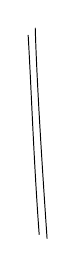
\begin{tikzpicture}[x=1mm,y=1mm,baseline=(current bounding box.center),line cap=round]
\draw[line width=0.35pt] (0,25.8) .. controls (0.4,19) and (0.7,10) .. (1.4,0.5);
\draw[line width=0.35pt] (0.9,26.7) .. controls (1.1,19.7) and (1.8,8.8) .. (2.4,0);
\end{tikzpicture}}
for \(\unsure{\Omega}=\mathbb C\)
\illegible{2} \unsure{comes down to}
\illegible{1} \uline{\unsure{orientation|orientations}} of
\illegible{1}}
But there remains the question whether this \deleted{\unsure{latter}}
\inserted{\unsure{\(\mu(u)\in\mu_n^*(\Omega)\)}}
can be deduced from knowledge at least of the
\inserted{outer} action of \(u\) on the group
``with \(1\) loop'' corresponding to the geometric situation
--- i.e. an \inserted{outer} automorphism
\deleted{\illegible{2}} of order \(n\) \unsure{of} such a group
(or whether here again one must decidedly regard it as an additional
datum).
\margin{yes, it can, thanks to the consideration of the
``subgroups \illegible{2} of \(\mathcal E\)''
\illegible{2} which define extensions
\diagram{\begin{tikzcd}[ampersand replacement=\&,row sep=2.5em,column sep=2em]
\unsure{1} \arrow[r] \& T \arrow[r] \arrow[dr,dotted,no head,"\unsure{n_i\,\mathrm{id}_T}"'] \& \mathcal E_i \arrow[r] \arrow[d,phantom,"\simeq"{description,rotate=90}] \& \Gamma_i \arrow[r] \& 1 \\
\& \& T \& \&
\end{tikzcd}}
whence \(\unsure{\Gamma_i\simeq T/n_iT}\)
\illegible{2}}
But if this were indeed so, it would imply on the other hand that the
construction of \unsure{\(u\in\) group|these groups} with

\margin{158}

\scanpage{160}

(1) loop(s), with the operation of \(\Gamma\) on it, cannot be carried out
either with the help of the mere \deleted{\illegible{2}}
knowledge of the action of \(\Gamma\) (\(=\mathbb Z/n\mathbb Z\))
on \(\pi\).
It is this question of ``drilling holes'' that we must therefore in the end,
at the very end, tackle!

As for the question of whether
\deleted{\illegible{1}}\inserted{in}
\deleted{\illegible{1}} the \uline{anabelian case},
the map
\[
\mu:\underbrace{{}_\infty\mathcal E}_{
\substack{\text{\unsure{set of}}\\
\text{\unsure{elements}}\\
\text{of finite order in }\mathcal E}}
\longrightarrow T\otimes\mathbb Q/\mathbb Z)
\]
is deducible from the action of \(\Gamma\) on \(\pi\)
[if it is faithful, \(\mathcal E\) is thus identified with a subgroup
of \(\operatorname{Autext}_{\unsure{\ell|l}}(\pi)\)
and we may ask whether \(\mu\) is not
\inserted{then} definable on this in its entirety],
or \unsure{it is|whether it is} an additional datum one must have in order to
reconstruct the geometric situation --- the question remains entirely open.
\margin{this does indeed seem \unsure{so}, taking into account
\illegible{1} that for \(\Gamma\) \uline{solvable},
\illegible{3}, we know \illegible{1}
that every action \deleted{\illegible{1}} of \(\Gamma\) on \(\pi\)
\illegible{3} \unsure{realize geometrically}}

\textcircled{16}\quad
\uuline{Plugging and drilling holes:}
General \unsure{topos-theoretic} \uline{preliminaries}

Let us consider a situation
\diagram{
\begin{tikzcd}
B_{D^*} \arrow[r] & B_U
\end{tikzcd}
}
(of multi-Galois topoi)
\margin{N.B. such a situation
\inserted{of topoi \unsure{describes}} \(2\)-faithfully the topological situations \((X,S)\),
or \(U\), provided that no irreducible component of \(U\)
is \(\simeq S^2\) ---}

\margin{159}
